\documentclass[final,11pt]{article}
\usepackage[T1]{fontenc}
\usepackage[english]{babel}
\usepackage[utf8]{inputenc}
\usepackage{graphicx}
\usepackage[activate={true,nocompatibility},final,tracking=true,kerning=true,spacing=true,factor=1100,stretch=10,shrink=10]{microtype}
\microtypecontext{spacing=nonfrench}
\usepackage{appendix}
\usepackage{caption}
\usepackage{enumerate}
\usepackage{amsthm}
\usepackage{tikz}
\usepackage{pgfplots}
\pgfplotsset{compat=1.18}
\usepackage[section]{placeins}
\usepackage[square,numbers]{natbib}
\usepackage[margin=1in]{geometry}
\usepackage[hidelinks]{hyperref}
\usepackage[fancy,section]{alex}

\hypersetup{
    pdftitle={The Bernoulli Hash Function: Optimal Bernoulli Sets and Bernoulli Maps},
    pdfauthor={Alexander Towell},
    pdfsubject={computer science},
    pdfkeywords={
        approximate sets,
        approximate maps,
        hash function,
        random oracle,
        Bernoulli set,
        Bernoulli map,
        Bernoulli hash function},
    colorlinks=false,
    citecolor=green,
    filecolor=magenta,
    urlcolor=green
}

% Paper-specific definitions for the Bernoulli Hash Function paper.
% General notation is provided by alex.sty.

%% Probability mass function (not in alex.sty)
\NewDocumentCommand{\PDF}{mO{}}{%
    \ifx\\#2\\%
        \operatorname{f}\!\left(#1\right)%
    \else%
        \operatorname{f}_{#2}\!\left(#1\right)%
    \fi%
}

%% Concatenation operator (alias for \cat from alex.sty, used in text)
\newcommand{\catop}{\cat}

%% Bit string notation
\newcommand{\cisb}{\BitSet^{*}}
\newcommand{\cisbn}[1]{\BitSet^{#1}}

%% Indicator function
\newcommand{\indicator}[1]{\mathbbm{1}_{#1}}

%% Ordinal helpers
\newcommand{\ith}{$i^{\text{th}}$}
\newcommand{\jth}{$j^{\text{th}}$}
\newcommand{\kth}{$k^{\text{th}}$}
\newcommand{\nth}{$n^{\text{th}}$}

%% Algorithm2e function keywords
\SetKwFunction{MakeBHF}{MakeBHF}
\SetKwFunction{Contains}{Contains}
\SetKwFunction{HasKey}{HasKey}
\SetKwFunction{Encode}{encode}
\SetKwFunction{Decode}{decode}
\SetKwFunction{ro}{$h^*$}
\SetKwFunction{sampler}{BitLengthSampler}
\SetKwFunction{Cardinality}{cardinality}
\SetKwFunction{Count}{count}
\SetKwFunction{FalsePositiveRate}{false\_positive\_rate}

%% Algorithm2e data keywords
\SetKwData{collisions}{collisions}

%% Algorithm styling
\definecolor{ltgray}{rgb}{0.6,0.6,0.6}
\newcommand\mycommfont[1]{\footnotesize\ttfamily\textcolor{ltgray}{#1}}
\SetCommentSty{mycommfont}

%% TikZ libraries
\usetikzlibrary{arrows,shapes,positioning}
\usetikzlibrary{calc,decorations.markings}

%% Graphics path
\graphicspath{{img/}}

%% Null value for maps
\newcommand{\nullvalue}{\bot}


\title{The Bernoulli Hash Function:\\Optimal Bernoulli Sets and Bernoulli Maps}
\author{
    Alexander Towell\\
    \texttt{atowell@siue.edu}
}
\date{}

\begin{document}
\maketitle

\begin{abstract}
We introduce the \emph{Bernoulli Hash Function} (BHF), a family of hash-based
constructions that optimally implement the Bernoulli set and Bernoulli map
abstract data types.
The BHF is parameterized by an \emph{acceptance predicate} over hash outputs:
the classical equality test $h(x \cat b) = h_0$ is a special case of a
generalized threshold test $h(x \cat b) \bmod N \leq t$, which provides
finer false positive rate granularity and eliminates the combinatorial subset
enumeration required when the false negative rate $\fnrate > 0$.
We also introduce an \emph{adaptive threshold} variant that sets $t$ to the
$p$-th order statistic of the hash residues, eliminating the salt search
entirely for sets and achieving $\mathcal{O}(\log N / m) \to 0$ bits per
element---at the cost of a random (Beta-distributed) false positive rate.
We prove that the BHF achieves the information-theoretic lower bound on space
complexity while maximizing entropy, for both sets (value length $\mu = 0$)
and maps (arbitrary $\mu$), under both predicate forms.
The construction is unified: the Bernoulli set is the special case of the
Bernoulli map with zero-length values, so a single framework and a single
space-optimality proof covers both.
\end{abstract}

\microtypesetup{protrusion=false}
\tableofcontents
\microtypesetup{protrusion=true}

\section{Introduction}
\label{sec:intro}

The Bernoulli set~\cite{bernoulli_sets} and Bernoulli map~\cite{bernoulli_maps}
are abstract data types that model sets and maps with quantifiable random errors.
A Bernoulli set $\ASet{S}$ of a set $\Set{S}$ tests each element independently:
negatives test positive with probability $\fprate$ (false positive rate) and
positives test negative with probability $\fnrate$ (false negative rate), each as
independent Bernoulli trials.
A Bernoulli map $\ASet{M}$ extends this to key-value pairs: the key domain
behaves as a Bernoulli set, and each positive key maps to its associated value.

This paper addresses the \emph{implementation} question: given a finite set or
map, how do we construct a space-optimal Bernoulli set or map with maximum
entropy?
We introduce the \emph{Bernoulli Hash Function} (BHF), a family of hash-based
constructions parameterized by an \emph{acceptance predicate} over hash
outputs.

\subsection*{Contributions}

We make three contributions:

\begin{enumerate}
    \item \textbf{Unified construction.}
    We present a single construction that implements both Bernoulli sets and
    Bernoulli maps.
    The set is the special case where the mean value bit length $\mu = 0$.
    One proof of space-optimality covers both.

    \item \textbf{Generalized acceptance predicate.}
    We generalize the membership predicate from an equality test
    ($h(x \cat b) = h_0$, yielding $\fprate \in \{2^{-k}\}$) to a threshold
    test ($h(x \cat b) \bmod N \leq t$, yielding
    $\fprate \in \{j/N : j = 1,\ldots,N\}$).
    The threshold test provides finer FPR granularity and, crucially,
    eliminates the $\binom{m}{p}$ subset enumeration when $\fnrate > 0$.
    We further introduce an \emph{adaptive} variant that sets $t$ to the
    $p$-th order statistic of the hash residues, eliminating the salt search
    entirely for sets (success probability 1) at the cost of a random FPR.

    \item \textbf{Information-theoretic optimality.}
    We prove that the BHF achieves the information-theoretic lower bound on
    space complexity while maximizing the entropy of its binary representation,
    under both predicate forms and for both sets and maps.
\end{enumerate}

\subsection*{Relation to companion papers}

The algebraic properties of Bernoulli sets (union, intersection, complement,
error propagation) are developed in~\cite{bernoulli_sets}.
The Bernoulli map algebra (composition, domain/codomain error) is
in~\cite{bernoulli_maps}.
The type-theoretic generalization is in~\cite{bernoulli_data_type}.
This paper focuses exclusively on \emph{constructing} optimal implementations
and cites those companions for the abstract theory.

\subsection*{Organization}

\Cref{sec:prelim} establishes notation and recalls the Bernoulli set and map
definitions.
\Cref{sec:shf} introduces the Bernoulli Hash Function family and the
generalized acceptance predicate.
\Cref{sec:construction} gives the construction algorithms.
\Cref{sec:space} proves space optimality.
\Cref{sec:entropy} analyzes the entropy properties.
\Cref{sec:prob_model} summarizes the probabilistic model.
\Cref{sec:operations} describes set operations on BHF instances.
\Cref{sec:discussion} discusses applications, obliviousness, and comparisons
with existing data structures.

\section{Preliminaries}
\label{sec:prelim}

\subsection{Bit strings and encoding}

The binary set is $\BitSet = \{0,1\}$.
The set of all bit strings of length $n$ is $\cisbn{n}$, with
$\Card{\cisbn{n}} = 2^n$.
The countably infinite set of all finite bit strings is
$\cisb = \bigcup_{n=0}^{\infty} \cisbn{n}$.
The bit length of an object $x$ is denoted $\BL(x)$.

\begin{definition}[Bit string--natural number bijection]
\label{def:mapping}
Let $\cisb$ and $\NatSet$ have the bijection
\begin{equation}
    (b_1 \, b_2 \, \cdots \, b_m) \longleftrightarrow 2^m + \sum_{j=1}^{m} 2^{m-j} b_j\,.
\end{equation}
We denote the image of a bit string (or natural number) $x$ under this
bijection by $x'$.
A natural number $n$ maps to a bit string of length $\lfloor \log_2 n \rfloor$.
\end{definition}

\subsection{Hash functions and the random oracle}

\begin{definition}[Hash function]
A \emph{hash function} $\hash \colon \cisb \to \cisbn{n}$ maps arbitrary-length
bit strings to fixed-length bit strings of length $n$.
\end{definition}

\begin{definition}[Random oracle]
\label{def:randomoracle}
A \emph{random oracle} $\ro \colon \cisb \to \cisbn{\infty}$ is a theoretical
hash function whose output is uniformly distributed over its range for every
unique input.
For any prefix length $k$, the first $k$ bits of $\ro(x)$ are uniformly
distributed over $\cisbn{k}$.
\end{definition}

\begin{assumption}[Random oracle approximation]
\label{asm:ro_approx}
The hash function $\hash$ approximates a random oracle $\ro$ and has a space
complexity of $\mathcal{O}(1)$.
\end{assumption}

\subsection{Bernoulli sets}
\label{sec:prelim_bset}

We recall the essential definitions from~\cite{bernoulli_sets}.

\begin{definition}[Bernoulli set]
\label{def:bernoulli_set}
Let $\Set{S} \subseteq \Set{U}$ be a finite set drawn from a universe
$\Set{U}$.
A \emph{Bernoulli set} $\ASet{S}$ of $\Set{S}$ with false positive rate
$\fprate$ and false negative rate $\fnrate$ satisfies:
\begin{enumerate}[(i)]
    \item For each $x \in \Set{S}$, independently,
    $\Prob{x \notin \ASet{S}} = \fnrate$.
    \item For each $x \in \Set{U} \setminus \Set{S}$, independently,
    $\Prob{x \in \ASet{S}} = \fprate$.
\end{enumerate}
A Bernoulli set with $\fnrate = 0$ is a \emph{positive} Bernoulli set,
denoted $\PASet{S}$.
A Bernoulli set with $\fprate = 0$ is a \emph{negative} Bernoulli set,
denoted $\NASet{S}$.
\end{definition}

\begin{postulate}[Space lower bound for sets]
\label{post:set_lb}
The optimal space complexity for a Bernoulli set over a countably infinite
universe is
\begin{equation}
    -(1 - \fnrate) \log_2 \fprate \;\; \si{bits \per element}\,.
\end{equation}
\end{postulate}

\subsection{Bernoulli maps}
\label{sec:prelim_bmap}

We recall the essential definitions from~\cite{bernoulli_maps}.

\begin{definition}[Bernoulli map]
\label{def:bernoulli_map}
Let $\Set{M} \subseteq \Set{X} \times \Set{Y}$ be a finite map (set of
key-value pairs where each key appears at most once).
A \emph{Bernoulli map} $\ASet{M}$ of $\Set{M}$ with false positive rate
$\fprate$ and false negative rate $\fnrate$ satisfies:
\begin{enumerate}[(i)]
    \item The key domain of $\ASet{M}$ is a Bernoulli set of the key domain
    of $\Set{M}$ with rates $\fprate$ and $\fnrate$.
    \item For each positive key $x$, $\Find(\ASet{M}, x)$ returns the correct
    value $\Set{M}[x]$.
    \item For each false-positive key $x$, $\Find(\ASet{M}, x)$ returns a
    value that is effectively random.
\end{enumerate}
\end{definition}

\begin{postulate}[Space lower bound for maps]
\label{post:map_lb}
The optimal space complexity for a Bernoulli map over a countably infinite key
universe, with mean value encoding length $\mu$ bits, is
\begin{equation}
    -(1 - \fnrate) \log_2 \fprate + (1-\fnrate)\mu \;\; \si{bits \per element}\,.
\end{equation}
\end{postulate}

\begin{remark}
Setting $\mu = 0$ in \cref{post:map_lb} recovers the set lower bound
(\cref{post:set_lb}).
This duality---the set as a degenerate map---is the organizing principle of
this paper.
\end{remark}

\section{The Bernoulli Hash Function family}
\label{sec:shf}

The \emph{Bernoulli Hash Function} (BHF) is a family of constructions that
encode a finite set or map into a compact binary representation using a hash
function and a \emph{salt}---a bit string $b$ discovered by search.
The key idea is an \emph{acceptance predicate} that determines membership.

\subsection{Acceptance predicates}

\begin{definition}[Acceptance predicate]
\label{def:acceptance}
Given a hash function $\hash$, a salt $b \in \cisb$, a modulus $N \in \NatSet$,
and an \emph{acceptance set} $\Set{A} \subseteq \{0, 1, \ldots, N-1\}$, an
element $x$ is \emph{accepted} if and only if
\begin{equation}
    \hash(x \cat b) \bmod N \in \Set{A}\,.
\end{equation}
Under the random oracle assumption (\cref{asm:ro_approx}), the false positive
rate is
\begin{equation}
    \fprate = \frac{\Card{\Set{A}}}{N}\,.
\end{equation}
\end{definition}

Two important special cases arise from the choice of $\Set{A}$:

\paragraph{Equality predicate (classical BHF).}
Set $N = 2^k$ and $\Set{A} = \{h_0\}$ for some $h_0 \in \{0,\ldots,2^k-1\}$
discovered adaptively during construction.
Then $\fprate = 2^{-k}$ and the membership test is
\begin{equation}
    \hash(x \cat b) \bmod 2^k = h_0\,.
\end{equation}
The achievable false positive rates are $\fprate \in \{2^{-k} : k \in \NatSet\}$.

\paragraph{Threshold predicate (generalization).}
Set $\Set{A} = \{0, 1, \ldots, t\}$ for a threshold $t \geq 0$.
Then $\fprate = (t+1)/N$ and the membership test is
\begin{equation}
\label{eq:threshold_test}
    \hash(x \cat b) \bmod N \leq t\,.
\end{equation}
The achievable false positive rates are
$\fprate \in \{j/N : j = 1, \ldots, N\}$, which is a much finer lattice
than the power-of-two constraint of the equality predicate.

\subsection{Success probability per trial}

The probability that a candidate salt $b$ produces a valid BHF depends on the
predicate type.

\begin{theorem}[Success probability---equality predicate]
\label{thm:success_eq}
For the equality predicate with $m$ keys, false positive rate
$\fprate = 2^{-k}$, and mean value encoding length $\mu$ bits, the probability
that a given salt $b$ yields a valid construction is
\begin{equation}
    p_{\mathrm{eq}}(m, \fprate, \mu) = \frac{\fprate^{m-1}}{2^{m\mu}}\,.
\end{equation}
\end{theorem}
\begin{proof}
Under the random oracle assumption, the hash of each key concatenated with
$b$ is independent and uniform.
The first key fixes the target hash $h_0$; each of the remaining $m-1$ keys
must hash to $h_0$, each with probability $\fprate$.
Additionally, for a map, each key's value must match the first $\BL(v_i)$ bits
of a second hash, contributing a factor of $2^{-\BL(v_i)}$ per key.
The product is
\begin{equation}
    \fprate^{m-1} \cdot \prod_{i=1}^{m} 2^{-\BL(v_i)}
    = \frac{\fprate^{m-1}}{2^{m\mu}}\,,
\end{equation}
where $\mu = \frac{1}{m}\sum_{i=1}^{m} \BL(v_i)$ is the mean value bit length.
For sets, $\mu = 0$ and the expression reduces to $\fprate^{m-1}$.
\end{proof}

\begin{theorem}[Success probability---threshold predicate]
\label{thm:success_thresh}
For the threshold predicate with modulus $N$, threshold $t$, $m$ keys, and mean
value encoding length $\mu$ bits, the probability that a given salt $b$ yields
a valid construction is
\begin{equation}
    p_{\mathrm{th}}(m, \fprate, \mu) = \frac{\fprate^{m}}{2^{m\mu}}\,.
\end{equation}
\end{theorem}
\begin{proof}
With the threshold predicate, the acceptance set $\Set{A} = \{0,\ldots,t\}$ is
fixed \emph{before} examining the salt.
Each of the $m$ keys must independently hash into $\Set{A}$, each with
probability $\fprate = (t+1)/N$.
This gives $\fprate^m$ (not $\fprate^{m-1}$, since no key is ``free'' to fix
the target).
The value-matching factor contributes $2^{-m\mu}$ as before.
\end{proof}

\begin{remark}
The equality predicate has a factor-of-$\fprate^{-1}$ advantage in success
probability because one key adaptively determines $h_0$.
In the space complexity (\cref{sec:space}), this manifests as an additive
$\log_2 \fprate / m$ bits per element, which vanishes as $m \to \infty$.
Both predicates achieve the same asymptotic optimum.
\end{remark}

\subsection{FPR granularity}

\begin{theorem}[FPR granularity]
\label{thm:fpr_granularity}
With modulus $N$, the threshold predicate achieves any false positive rate in
the lattice
\begin{equation}
    \fprate \in \left\{\frac{j}{N} : j = 1, 2, \ldots, N\right\}\,,
\end{equation}
whereas the equality predicate achieves only
$\fprate \in \{2^{-k} : k \in \NatSet\}$.
\end{theorem}

This is immediate from the definitions.
For example, with $N = 100$, one can achieve $\fprate = 0.01, 0.02, \ldots, 1.00$, whereas the equality predicate can only achieve $\fprate = 0.5, 0.25, 0.125, \ldots$

\subsection{Simplified search for $\fnrate > 0$}

When the false negative rate $\fnrate > 0$, only $p = (1-\fnrate)m$ of the
$m$ elements need to be accepted.
Under the equality predicate, the algorithm must enumerate all $\binom{m}{p}$
subsets of size $p$ and check whether each subset collides.
Under the threshold predicate, the search is dramatically simpler.

\begin{theorem}[Search complexity for $\fnrate > 0$]
\label{thm:fnr_search}
Under the threshold predicate, testing whether a candidate salt $b$ admits at
least $p$ of $m$ elements requires $\mathcal{O}(m)$ hash evaluations: simply
count how many elements satisfy $\hash(x \cat b) \bmod N \leq t$.

Under the equality predicate, the same test requires
$\mathcal{O}\!\left(\binom{m}{p} \cdot m\right)$ hash evaluations in the worst
case, since each candidate $h_0$ (determined by each $p$-subset) must be
checked against all elements.
\end{theorem}
\begin{proof}
For the threshold predicate, the acceptance set $\Set{A}$ is fixed.
For each candidate salt $b$, we compute $\hash(x_i \cat b) \bmod N$ for
$i = 1,\ldots,m$ and count the number that fall in $\Set{A}$.
If at least $p$ do, the salt succeeds.
This is $\mathcal{O}(m)$ per candidate salt.

For the equality predicate, the target $h_0$ is not known a priori.
For each $p$-element subset, the first element determines $h_0$, and the
remaining $p-1$ elements must match.
Since there are $\binom{m}{p}$ such subsets, the worst-case cost per candidate
salt is $\mathcal{O}\!\left(\binom{m}{p} \cdot m\right)$.
\end{proof}

\subsection{Adaptive threshold}
\label{sec:adaptive}

The equality and threshold predicates both fix the acceptance set \emph{before}
examining the data, then search for a salt that maps all (or enough) elements
into it.
An alternative is to let the data \emph{determine} the threshold.

\begin{definition}[Adaptive threshold predicate]
\label{def:adaptive_threshold}
Given a salt $b \in \cisb$, a modulus $N$, and $m$ keys
$x_1,\ldots,x_m$, compute the residues
\begin{equation}
    r_i \;=\; \hash(x_i \cat b) \bmod N\,, \quad i = 1,\ldots,m\,,
\end{equation}
and let $\OS{p}{m}$ denote the $p$-th order statistic (the $p$-th smallest
value among $r_1,\ldots,r_m$).
Set the threshold $t = \OS{p}{m}$.
An element $x$ is accepted if and only if
\begin{equation}
\label{eq:adaptive_test}
    \hash(x \cat b) \bmod N \leq t\,.
\end{equation}
By construction, at least $p$ of the $m$ keys are accepted.
The false positive rate is the random variable
\begin{equation}
\label{eq:adaptive_fpr}
    \fprate \;=\; \frac{\OS{p}{m} + 1}{N}\,.
\end{equation}
\end{definition}

\begin{remark}
Unlike the fixed-threshold predicate, the adaptive threshold produces a
\emph{random} false positive rate that depends on the particular salt and keys.
The parameter $p$ controls the expected FPR: choosing
$p = \lfloor \epsilon^{*}(m+1) \rfloor$ targets a desired mean FPR of
$\epsilon^{*}$.
\end{remark}

\subsubsection{Success probability}

\begin{theorem}[Success probability---adaptive threshold, sets]
\label{thm:success_adaptive_set}
For the adaptive threshold predicate applied to a Bernoulli set ($\mu = 0$)
with $m$ keys and $p \leq m$, every candidate salt $b$ yields a valid
construction.
The success probability per trial is
\begin{equation}
    p_{\mathrm{ad}} = 1\,.
\end{equation}
\end{theorem}
\begin{proof}
For any salt $b$, the $m$ residues $r_1,\ldots,r_m$ are well-defined.
We sort them and set $t = \OS{p}{m}$.
By the definition of the $p$-th order statistic, at least $p$ residues
satisfy $r_i \leq t$.
Since there is no value-matching constraint ($\mu = 0$), every salt succeeds.
No search is required.
\end{proof}

\begin{theorem}[Success probability---adaptive threshold, maps]
\label{thm:success_adaptive_map}
For the adaptive threshold predicate applied to a Bernoulli map ($\mu > 0$)
with $m$ keys and value encoding lengths $\BL(v_1),\ldots,\BL(v_m)$, the
success probability per trial is
\begin{equation}
\label{eq:success_adaptive_map}
    p_{\mathrm{ad}}(m, p, \mu)
    \;=\; \Prob{\Card{\Set{V}} \geq p}\,,
\end{equation}
where $\Set{V} = \{i : \hash(1 \cat x_i \cat b) \bmod 2^{\BL(v_i)} =
\Encode(v_i)\}$ is the set of value-matching keys and
$\Card{\Set{V}} \sim \bindist(m, 2^{-\mu})$ under the random oracle
assumption.
\end{theorem}
\begin{proof}
The value-matching constraint is independent of the residue ordering.
For each key $x_i$, the value hash matches with probability $2^{-\BL(v_i)}$.
Under the random oracle assumption, these are independent Bernoulli trials, so
$\Card{\Set{V}} \sim \bindist(m, 2^{-\mu})$ (exactly when all values have the
same encoding length; approximately otherwise).
The adaptive threshold can be set on any $p$ of the value-matching keys, so the
salt succeeds if and only if $\Card{\Set{V}} \geq p$.
\end{proof}

\begin{corollary}
\label{cor:adaptive_no_search}
For Bernoulli sets, the adaptive threshold eliminates the salt search entirely:
the first (and only) candidate salt $b$ always succeeds.
The construction time is $\mathcal{O}(m \log m)$ (dominated by sorting the
residues).
\end{corollary}

\subsubsection{FPR distribution}

Under the random oracle assumption, the residues $r_1,\ldots,r_m$ are i.i.d.\
uniform on $\{0,1,\ldots,N-1\}$.
The threshold $t = \OS{p}{m}$ is therefore the $p$-th order statistic of $m$
i.i.d.\ discrete uniform random variables.

\begin{theorem}[Exact FPR distribution]
\label{thm:fpr_distribution}
For sets ($\mu = 0$), the threshold $T = \OS{p}{m}$ has the probability mass
function
\begin{equation}
\label{eq:os_pmf}
    \Prob{T = j}
    \;=\; \frac{\binom{j}{p-1}\binom{N-1-j}{m-p}}{\binom{N-1}{m-1}}
    \cdot \frac{m}{N}\,,
    \quad j = p-1, p, \ldots, N-1-(m-p)\,,
\end{equation}
which is the PMF of the $p$-th order statistic from $m$ i.i.d.\
$\operatorname{Uniform}\{0,\ldots,N-1\}$ draws.
Equivalently, $T + 1$ follows a
$\operatorname{BetaBinomial}(N, p, m - p + 1)$ distribution shifted by $p$.

In the continuous limit ($N \to \infty$ with $\fprate = (T+1)/N$), the FPR
converges in distribution:
\begin{equation}
\label{eq:fpr_beta}
    \fprate \;\xrightarrow{d}\; \betadist(p,\; m - p + 1)\,.
\end{equation}
\end{theorem}
\begin{proof}
See \cref{sec:adaptive_pmf_derivation} for the exact discrete derivation.
The continuous limit follows from the classical result that the $p$-th order
statistic of $m$ i.i.d.\ $\operatorname{Uniform}(0,1)$ random variables has
a $\betadist(p, m - p + 1)$
distribution~\cite{order_statistics}.
\end{proof}

\begin{theorem}[Moments of the adaptive FPR]
\label{thm:adaptive_moments}
In the continuous limit, the expected FPR and its variance are
\begin{align}
\label{eq:adaptive_mean}
    \Expect{\fprate} &= \frac{p}{m + 1}\,, \\
\label{eq:adaptive_var}
    \Var{\fprate} &= \frac{p(m - p + 1)}{(m + 1)^2(m + 2)}\,.
\end{align}
To target a desired mean FPR of $\epsilon^{*}$, choose
\begin{equation}
\label{eq:adaptive_p_choice}
    p = \lfloor \epsilon^{*}(m + 1) \rfloor\,.
\end{equation}
The variance $\Var{\fprate} = \mathcal{O}(1/m)$ vanishes as $m \to \infty$,
so the FPR concentrates around $\epsilon^{*}$.
\end{theorem}
\begin{proof}
These are the moments of the $\betadist(p, m - p + 1)$ distribution:
$\Expect{X} = \alpha / (\alpha + \beta)$ and
$\Var{X} = \alpha\beta / ((\alpha + \beta)^2(\alpha + \beta + 1))$
with $\alpha = p$ and $\beta = m - p + 1$.
\end{proof}

\begin{remark}
For maps ($\mu > 0$), the FPR distribution is a mixture: conditioned on the
number of value-matching keys $\Card{\Set{V}} = v \geq p$, the threshold is the
$p$-th order statistic of $v$ residues.
The unconditional FPR is
\begin{equation}
    \fprate \mid \Card{\Set{V}} = v \;\sim\; \betadist(p, v - p + 1)\,,
\end{equation}
and the marginal FPR averages over $\Card{\Set{V}} \sim \bindist(m, 2^{-\mu})$
restricted to $\Card{\Set{V}} \geq p$.
\end{remark}

\subsubsection{Search complexity}

\begin{theorem}[Construction complexity---adaptive threshold]
\label{thm:adaptive_complexity}
The construction time for the adaptive threshold predicate is:
\begin{enumerate}[(i)]
    \item Sets ($\mu = 0$): $\mathcal{O}(m \log m)$ (one pass, dominated by
    sorting the $m$ residues).
    \item Maps ($\mu > 0$): Expected $\mathcal{O}(m \log m / p_{\mathrm{ad}})$,
    where $p_{\mathrm{ad}} = \Prob{\Card{\Set{V}} \geq p}$.
    Each trial costs $\mathcal{O}(m \log m)$ and the expected number of trials
    is $1 / p_{\mathrm{ad}}$.
\end{enumerate}
\end{theorem}
\begin{proof}
For sets, the construction hashes $m$ elements ($\mathcal{O}(m)$), sorts the
residues ($\mathcal{O}(m \log m)$), and reads off $t = \OS{p}{m}$.
No search is needed (\cref{thm:success_adaptive_set}).

For maps, each candidate salt requires $\mathcal{O}(m)$ hash evaluations to
identify value-matching keys and $\mathcal{O}(m \log m)$ to sort residues.
The geometric search terminates after an expected $1/p_{\mathrm{ad}}$ trials.
\end{proof}

\subsubsection{Comparison of predicates}

\begin{table}[ht]
\centering
\caption{Comparison of the three acceptance predicates for the BHF.}
\label{tab:predicate_comparison}
\begin{tabular}{lccc}
\hline
 & \textbf{Equality} & \textbf{Threshold} & \textbf{Adaptive} \\
\hline
FPR type & fixed & fixed & random \\
FPR values ($\mu=0$) & $\{2^{-k}\}$ & $\{j/N\}$ & $\betadist(p,m\!-\!p\!+\!1)$ \\
Success prob.\ (sets) & $\fprate^{m-1}$ & $\fprate^{m}$ & $1$ \\
Salt search & geometric & geometric & none (sets) \\
Construction & $\mathcal{O}(m/p)$ trials & $\mathcal{O}(m/p)$ trials & $\mathcal{O}(m \log m)$ \\
Stored params & $(h_k, b)$ & $(N, t, b)$ & $(N, t)$ \\
Bits/element & $-\!\log_2\!\fprate + \mu$ & $-\!\log_2\!\fprate + \mu$ & $\mathcal{O}(\log N / m)$ \\
Max entropy? & yes & yes & no (see \cref{sec:adaptive_entropy}) \\
\hline
\end{tabular}
\end{table}

\subsubsection{Adaptive FPR distribution}

\Cref{fig:adaptive_fpr} shows the $\betadist(p, m - p + 1)$ density for
several choices of $(m, p)$.
As $m$ grows, the density concentrates around the mean $p/(m+1)$.

\begin{figure}[ht]
\centering
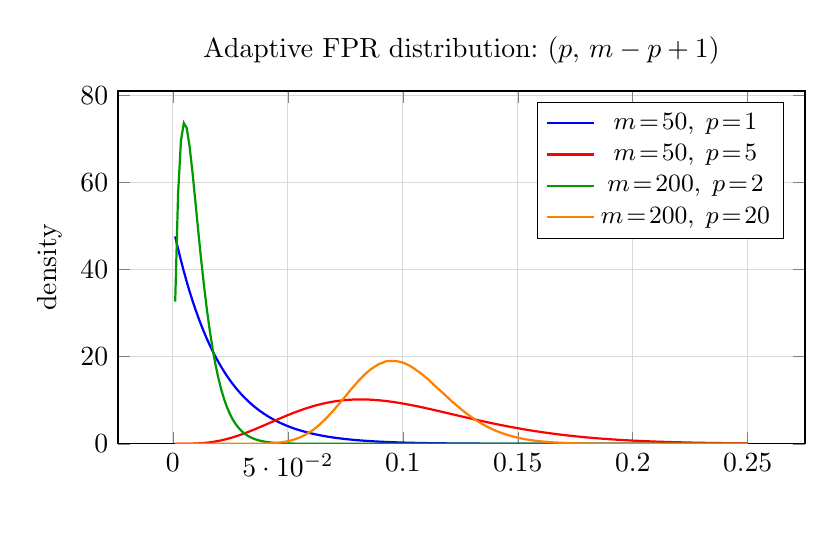
\begin{tikzpicture}
\begin{axis}[
    width=0.85\textwidth,
    height=0.5\textwidth,
    xlabel={$\fprate$},
    ylabel={density},
    domain=0.001:0.25,
    samples=200,
    legend style={at={(0.97,0.97)}, anchor=north east, font=\small},
    ymin=0,
    grid=major,
    grid style={gray!30},
    every axis plot/.append style={thick, no markers},
    title={Adaptive FPR distribution: $\betadist(p,\, m - p + 1)$}
]
% Beta PDF: f(x) = x^(a-1)(1-x)^(b-1) / B(a,b)
% We use pgfplots math; gamma function via ln(x!) trick not available,
% so we normalise visually using the known mode and scale.

% (m=50, p=1): Beta(1,50) -- exponential-like
\addplot[blue] {(1-x)^49 * 50};
\addlegendentry{$m\!=\!50,\; p\!=\!1$}

% (m=50, p=5): Beta(5,46)
\addplot[red] {x^4 * (1-x)^45 * 50! / (4! * 45!)};
\addlegendentry{$m\!=\!50,\; p\!=\!5$}

% (m=200, p=2): Beta(2,199)
\addplot[green!60!black] {x * (1-x)^198 * 200*199};
\addlegendentry{$m\!=\!200,\; p\!=\!2$}

% (m=200, p=20): Beta(20,181)
\addplot[orange] {
    exp(
        19*ln(x) + 180*ln(1-x)
        + ln(200!) - ln(19!) - ln(180!)
    )
};
\addlegendentry{$m\!=\!200,\; p\!=\!20$}

\end{axis}
\end{tikzpicture}
\caption{The $\betadist(p, m-p+1)$ density of the adaptive FPR for several
    $(m,p)$ pairs.
    As $m$ grows (green, orange curves), the density concentrates around the
    mean $\Expect{\fprate} = p/(m+1)$.
    For $p = 1$ (blue), the density is a decaying exponential concentrated near
    zero.}
\label{fig:adaptive_fpr}
\end{figure}

\section{Construction algorithms}
\label{sec:construction}

We present the unified construction that produces both Bernoulli sets ($\mu=0$)
and Bernoulli maps ($\mu > 0$).
We give versions for both the equality and threshold predicates, and the
membership/lookup queries.

\subsection{Map construction (general case)}

\begin{algorithm}[ht]
    \caption{Unified BHF construction (equality predicate)}
    \label{alg:make_shf_eq}
    \DontPrintSemicolon
    \SetKwProg{func}{function}{}{}
    \KwIn{
        $\Set{M} = \{(x_1,v_1),\ldots,(x_m,v_m)\}$ is a finite map
        (for a set, $v_i = \epsilon$ for all $i$),
        $\fprate = 2^{-k}$ is the false positive rate,
        $\fnrate$ is the maximum false negative rate.
    }
    \KwOut{
        A Bernoulli map $\ASet{M}$ coded as a tuple $(h_k, b)$.
    }
    \func{\MakeBHF{$\Set{M}$, $\fprate$, $\fnrate$}}{
        $p \gets \lceil (1 - \fnrate) \cdot m \rceil$
        \tcp*{minimum true positives}
        $k \gets -\log_2 \fprate$\;
        \For{$n \gets 0$ \KwTo $\infty$}{
            \For{$j \gets 1$ \KwTo $2^n$}{
                $b \gets$ draw a bit string of length $n$ uniformly at random
                    from $\cisbn{n}$ without replacement\;
                \tcp{Test all $\binom{m}{p}$ subsets of size $p$}
                \ForEach{subset $\Set{P} \subseteq \Set{M}$ with
                    $\Card{\Set{P}} = p$}{
                    Let $(x^{(1)},v^{(1)}),\ldots,(x^{(p)},v^{(p)})$
                        be the elements of $\Set{P}$\;
                    $h_k \gets \hash(x^{(1)} \cat b) \bmod 2^k$\;
                    $\found \gets \True$\;
                    \For{$i \gets 2$ \KwTo $p$}{
                        \If{$\hash(x^{(i)} \cat b) \bmod 2^k \neq h_k$}{
                            $\found \gets \False$\;
                            \Break\;
                        }
                        \tcp{For maps: check value match}
                        \If{$\mu > 0$ \textbf{and}
                            $\hash(1 \cat x^{(i)}) \bmod 2^{\BL(v^{(i)})}
                            \neq \Encode(v^{(i)})$}{
                            $\found \gets \False$\;
                            \Break\;
                        }
                    }
                    \If{\found}{
                        \Return $(h_k, b)$\;
                    }
                }
            }
        }
    }
\end{algorithm}

\begin{algorithm}[ht]
    \caption{Unified BHF construction (threshold predicate)}
    \label{alg:make_shf_th}
    \DontPrintSemicolon
    \SetKwProg{func}{function}{}{}
    \KwIn{
        $\Set{M} = \{(x_1,v_1),\ldots,(x_m,v_m)\}$ is a finite map,
        $N$ is the modulus,
        $t$ is the threshold ($\fprate = (t+1)/N$),
        $\fnrate$ is the maximum false negative rate.
    }
    \KwOut{
        A Bernoulli map $\ASet{M}$ coded as a tuple $(N, t, b)$.
    }
    \func{\MakeBHF{$\Set{M}$, $N$, $t$, $\fnrate$}}{
        $p \gets \lceil (1 - \fnrate) \cdot m \rceil$
        \tcp*{minimum true positives}
        \For{$n \gets 0$ \KwTo $\infty$}{
            \For{$j \gets 1$ \KwTo $2^n$}{
                $b \gets$ draw a bit string of length $n$ uniformly at random
                    from $\cisbn{n}$ without replacement\;
                $c \gets 0$
                \tcp*{count of accepted elements}
                \For{$i \gets 1$ \KwTo $m$}{
                    \If{$\hash(x_i \cat b) \bmod N \leq t$}{
                        \tcp{For maps: also check value match}
                        \If{$\mu = 0$ \textbf{or}
                            $\hash(1 \cat x_i) \bmod 2^{\BL(v_i)}
                            = \Encode(v_i)$}{
                            $c \gets c + 1$\;
                        }
                    }
                }
                \If{$c \geq p$}{
                    \Return $(N, t, b)$\;
                }
            }
        }
    }
\end{algorithm}

\begin{remark}
The threshold construction (\cref{alg:make_shf_th}) performs $\mathcal{O}(m)$
work per candidate salt, regardless of $\fnrate$.
The equality construction (\cref{alg:make_shf_eq}) requires
$\mathcal{O}\!\left(\binom{m}{p} \cdot p\right)$ work per candidate salt when
$\fnrate > 0$.
When $\fnrate = 0$, both reduce to $\mathcal{O}(m)$ per candidate.
\end{remark}

\begin{algorithm}[ht]
    \caption{Unified BHF construction (adaptive threshold predicate)}
    \label{alg:make_shf_adaptive}
    \DontPrintSemicolon
    \SetKwProg{func}{function}{}{}
    \KwIn{
        $\Set{M} = \{(x_1,v_1),\ldots,(x_m,v_m)\}$ is a finite map
        (for a set, $v_i = \epsilon$ for all $i$),
        $N$ is the modulus,
        $p$ is the number of elements to accept
        ($\fnrate = 1 - p/m$).
    }
    \KwOut{
        A Bernoulli map $\ASet{M}$ coded as a tuple $(N, t)$.
    }
    \func{\MakeBHFAdaptive{$\Set{M}$, $N$, $p$}}{
        \tcp{For sets ($\mu = 0$): any salt works; pick $b = \epsilon$}
        \uIf{$\mu = 0$}{
            $b \gets \epsilon$
            \tcp*{empty string---no search needed}
            Compute $r_i \gets \hash(x_i \cat b) \bmod N$ for $i = 1,\ldots,m$\;
            Sort $r_{(1)} \leq r_{(2)} \leq \cdots \leq r_{(m)}$\;
            $t \gets r_{(p)}$\;
            \Return $(N, t)$\;
        }
        \tcp{For maps ($\mu > 0$): search for a salt with $\geq p$
            value-matching keys}
        \For{$n \gets 0$ \KwTo $\infty$}{
            \For{$j \gets 1$ \KwTo $2^n$}{
                $b \gets$ draw a bit string of length $n$ uniformly at random
                    from $\cisbn{n}$ without replacement\;
                $\Set{V} \gets \emptyset$
                \tcp*{value-matching keys}
                \For{$i \gets 1$ \KwTo $m$}{
                    \If{$\hash(1 \cat x_i \cat b) \bmod 2^{\BL(v_i)}
                        = \Encode(v_i)$}{
                        $\Set{V} \gets \Set{V} \cup \{i\}$\;
                    }
                }
                \If{$\Card{\Set{V}} \geq p$}{
                    Compute $r_i \gets \hash(x_i \cat b) \bmod N$ for
                        $i \in \Set{V}$\;
                    Sort the residues $\{r_i : i \in \Set{V}\}$\;
                    $t \gets$ the $p$-th smallest residue\;
                    \Return $(N, t)$\;
                }
            }
        }
    }
\end{algorithm}

\begin{remark}
The adaptive construction (\cref{alg:make_shf_adaptive}) differs fundamentally
from the equality and threshold constructions: for sets ($\mu = 0$), no salt
search is required.
The salt can be fixed to the empty string $\epsilon$, and the entire
construction reduces to hashing, sorting, and reading off the $p$-th order
statistic.
The output $(N, t)$ does not include a salt, since it is not needed.
For maps, the search loop finds a salt with enough value-matching keys, then
the adaptive threshold is set on the matching subset.
\end{remark}

\subsection{Set construction as a special case}

For a Bernoulli set, each value $v_i$ is the empty string ($\mu = 0$).
The value-matching conditions in both algorithms are trivially satisfied,
and the construction reduces to finding a salt $b$ such that at least $p$
elements pass the acceptance predicate.

\subsection{Membership test and value lookup}

\begin{algorithm}[ht]
    \caption{Membership test (\protect\Contains)}
    \label{alg:contains}
    \DontPrintSemicolon
    \SetKwProg{func}{function}{}{}
    \KwIn{
        $\ASet{S}$ is an BHF-coded Bernoulli set with parameters
        $(h_k, b)$ or $(N, t, b)$, and $x$ is the query element.
    }
    \KwOut{
        \True if $x$ is accepted, \False otherwise.
    }
    \func{\Contains{$\ASet{S}$, $x$}}{
        \tcp{Equality predicate version:}
        \uIf{equality predicate}{
            \Return $\hash(x \cat b) \bmod 2^k = h_k$\;
        }
        \tcp{Threshold predicate version:}
        \uElse{
            \Return $\hash(x \cat b) \bmod N \leq t$\;
        }
    }
\end{algorithm}

\begin{algorithm}[ht]
    \caption{Value lookup (\protect\Find) for Bernoulli maps}
    \label{alg:find}
    \DontPrintSemicolon
    \SetKwProg{func}{function}{}{}
    \KwIn{
        $\ASet{M}$ is an BHF-coded Bernoulli map and $x$ is the query key.
    }
    \KwOut{
        If $x$ is a positive key, returns $\Set{M}[x]$.
        If $x$ is a false positive, returns a random value.
        Otherwise returns $\nullvalue$.
    }
    \func{\Find{$\ASet{M}$, $x$}}{
        \If{$\lnot\;\Contains(\ASet{M}, x)$}{
            \Return $\nullvalue$\;
        }
        $c \gets \hash(1 \cat x \cat b)$
        \tcp*{extract value bits}
        $({\rm success}, y) \gets \Decode(c)$\;
        \If{${\rm success}$}{
            \Return $y$\;
        }
        \Return $\nullvalue$\;
    }
\end{algorithm}

The encoding function $\Encode \colon \Set{Y} \to \cisb$ must be
\emph{self-delimiting} (prefix-free): the decoder can determine where the
encoding ends without external length information.
For a positive key, the hash of $1 \cat x \cat b$ was constrained during
construction to begin with $\Encode(v)$, so decoding succeeds.
For a false-positive key, the hash bits are effectively random, so decoding
may or may not succeed; if it does, the returned value is random.

\section{Space complexity}
\label{sec:space}

We prove that the BHF achieves the information-theoretic lower bound on space
complexity for both Bernoulli sets and Bernoulli maps, under both predicate
forms.

\subsection{General proof (maps)}

The BHF representation is the tuple $(h_k, b)$ or $(N, t, b)$.
The dominant term is the length of the salt $b$, which the algorithm discovers
by exhaustive search in order of increasing length.

\begin{theorem}[Success probability per trial]
\label{thm:success_prob}
The probability that a candidate salt $b$ yields a valid BHF for a map with
$m$ keys, false positive rate $\fprate$, and mean value encoding length $\mu$
is:
\begin{enumerate}[(i)]
    \item Equality predicate: $p_{\mathrm{eq}} = \fprate^{m-1} / 2^{m\mu}$.
    \item Threshold predicate: $p_{\mathrm{th}} = \fprate^{m} / 2^{m\mu}$.
\end{enumerate}
\end{theorem}
\begin{proof}
See \cref{thm:success_eq,thm:success_thresh}.
\end{proof}

\begin{theorem}[Space complexity of the BHF]
\label{thm:space}
The expected bit length of the BHF asymptotically achieves
\begin{equation}
    -\log_2 \fprate + \mu \;\; \si{bits \per element}
\end{equation}
as $m \to \infty$, for both predicate forms.
\end{theorem}
\begin{proof}
The algorithm searches through candidate salts in order of increasing bit
length.
By \cref{def:mapping}, the \nth candidate maps uniquely to a bit string.
The search terminates at the first success, which follows a geometric
distribution with parameter $p$ (where $p = p_{\mathrm{eq}}$ or
$p = p_{\mathrm{th}}$).

Let $\RV{Q} \sim \geodist(p)$ be the trial at which the first success occurs.
The salt bit length is $\RV{N} \approx \log_2 \RV{Q}$ (a slight overestimate
from dropping the floor).

We approximate $\Expect{\RV{N}}$ via a second-order Taylor expansion of
$\log_2$ around $\Expect{\RV{Q}}$:
\begin{equation}
    \Expect{\RV{N}} \approx \log_2 \Expect{\RV{Q}}
        - \frac{\log_2 e}{\Expect{\RV{Q}}} \Var{\RV{Q}}\,.
\end{equation}
For $\RV{Q} \sim \geodist(p)$, $\Expect{\RV{Q}} = 1/p$ and
$\Var{\RV{Q}} = (1-p)/p^2$.
Substituting:
\begin{equation}
    \Expect{\RV{N}} \approx -\log_2 p + (1 - 1/p) \log_2 e\,.
\end{equation}

\paragraph{Equality predicate.}
With $p = \fprate^{m-1}/2^{m\mu}$:
\begin{align}
    \Expect{\RV{N}}
        &\approx -(m-1)\log_2 \fprate + m\mu
            + (1 - \fprate^{-(m-1)} 2^{m\mu}) \log_2 e\,.
\end{align}
Dividing by $m$ and taking $m \to \infty$:
\begin{equation}
    \frac{\Expect{\RV{N}}}{m} \to -\log_2 \fprate + \mu\,.
\end{equation}

\paragraph{Threshold predicate.}
With $p = \fprate^{m}/2^{m\mu}$:
\begin{align}
    \Expect{\RV{N}}
        &\approx -m\log_2 \fprate + m\mu
            + (1 - \fprate^{-m} 2^{m\mu}) \log_2 e\,.
\end{align}
Dividing by $m$ and taking $m \to \infty$:
\begin{equation}
    \frac{\Expect{\RV{N}}}{m} \to -\log_2 \fprate + \mu\,.
\end{equation}
In both cases, the expected bits per element converges to the information-theoretic lower bound $-\log_2 \fprate + \mu$.
\end{proof}

\subsection{Set as corollary}

\begin{corollary}[Space complexity for sets]
\label{cor:set_space}
For a Bernoulli set ($\mu = 0$), the BHF achieves $-\log_2 \fprate$ bits per
element asymptotically.
\end{corollary}
\begin{proof}
Set $\mu = 0$ in \cref{thm:space}.
\end{proof}

\subsection{Finite-sample correction}

For finite $m$, the exact bits per element are:
\begin{equation}
    \frac{\Expect{\RV{N}}}{m} =
    \begin{cases}
        -\dfrac{m-1}{m}\log_2 \fprate + \mu + \mathcal{O}(1/m)
            & \text{(equality)}\,,\\[8pt]
        -\log_2 \fprate + \mu + \mathcal{O}(1/m)
            & \text{(threshold)}\,.
    \end{cases}
\end{equation}
The equality predicate is slightly more space-efficient for small $m$
(by $\log_2 \fprate / m$ bits per element) due to the adaptive $h_0$.

\subsection{Effect of false negatives}

When $\fnrate > 0$, only $p = (1-\fnrate)m$ elements need to be accepted.
The success probability becomes (for the equality predicate):
\begin{equation}
    p = \frac{\fprate^{p-1}}{2^{p\mu}}\,,
\end{equation}
and the space complexity per element of the \emph{original} set becomes:
\begin{equation}
    \frac{p}{m}\left(-\log_2 \fprate + \mu\right)
    = (1 - \fnrate)\left(-\log_2 \fprate + \mu\right)\,,
\end{equation}
matching the lower bound in \cref{post:map_lb}.

\subsection{Space complexity of the adaptive threshold}
\label{sec:adaptive_space}

The adaptive threshold stores the pair $(N, t)$ with no salt.
This yields dramatically lower per-element cost, but the FPR is a random
variable rather than a fixed parameter.

\begin{theorem}[Space complexity---adaptive threshold]
\label{thm:adaptive_space}
For a Bernoulli set ($\mu = 0$) with $m$ keys and modulus $N$, the adaptive
threshold BHF stores $(N, t)$ using
\begin{equation}
\label{eq:adaptive_bits}
    \lceil \log_2 N \rceil + \lceil \log_2 N \rceil
    \;=\; 2\lceil \log_2 N \rceil \;\;\si{bits}
\end{equation}
total (or $\lceil \log_2 N \rceil + \lceil \log_2(t+1) \rceil$ if $t$ is
encoded in fewer bits).
The per-element cost is
\begin{equation}
\label{eq:adaptive_per_element}
    \frac{2\lceil \log_2 N \rceil}{m} \;=\; \mathcal{O}\!\left(\frac{\log N}{m}\right) \;\to\; 0
    \quad\text{as } m \to \infty\,.
\end{equation}
\end{theorem}
\begin{proof}
The modulus $N$ requires $\lceil \log_2 N \rceil$ bits to encode, and the
threshold $t \in \{0,\ldots,N-1\}$ requires at most $\lceil \log_2 N \rceil$
bits.
There is no salt to store (for sets, $b = \epsilon$).
The per-element cost is the total divided by $m$, which vanishes as
$m \to \infty$ for any fixed $N$.
\end{proof}

\begin{remark}[Why zero per-element cost does not violate the lower bound]
\label{rem:lb_not_violated}
The information-theoretic lower bound of $-\log_2 \fprate + \mu$ bits per
element assumes a \emph{fixed, predetermined} false positive rate $\fprate$.
The adaptive threshold does not fix $\fprate$---it is a random variable
(\cref{thm:fpr_distribution}).
The lower bound applies to the \emph{worst-case} FPR realization, not to
the expected FPR.
More precisely, the adaptive threshold trades FPR
\emph{predictability} for space savings: instead of guaranteeing
$\fprate = \epsilon^{*}$, it guarantees only
$\Expect{\fprate} = p/(m+1) \approx \epsilon^{*}$, with the actual FPR
drawn from a $\betadist(p, m - p + 1)$ distribution whose variance is
$\mathcal{O}(1/m)$.
The ``missing'' $m(-\log_2\fprate)$ bits of information are encoded in the
randomness of $\fprate$ itself.
\end{remark}

\Cref{fig:space_comparison} compares the per-element space cost across the
three predicates.

\begin{figure}[ht]
\centering
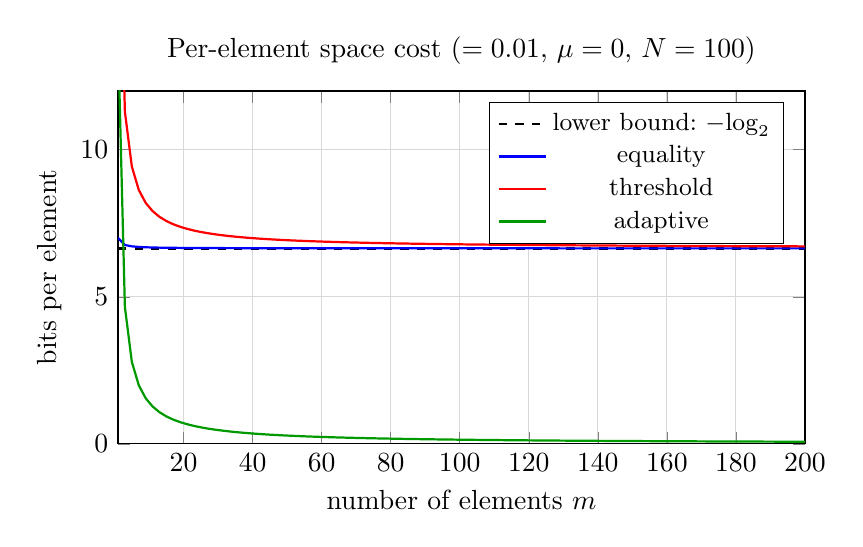
\begin{tikzpicture}
\begin{axis}[
    width=0.85\textwidth,
    height=0.5\textwidth,
    xlabel={number of elements $m$},
    ylabel={bits per element},
    xmin=1, xmax=200,
    ymin=0, ymax=12,
    legend style={at={(0.97,0.97)}, anchor=north east, font=\small},
    grid=major,
    grid style={gray!30},
    every axis plot/.append style={thick},
    title={Per-element space cost ($\fprate = 0.01$, $\mu = 0$, $N = 100$)}
]

% Lower bound: -log2(0.01) = 6.644
\addplot[black, dashed, domain=1:200, samples=100] {6.644};
\addlegendentry{lower bound: $-\!\log_2 \fprate$}

% Equality: -(m-1)/m * log2(eps) + O(1/m) ≈ (m-1)/m * 6.644 + log2(1/eps)/m
% success prob = eps^(m-1), salt bits ≈ (m-1)*log2(1/eps), plus k = log2(1/eps)
% total/m = (m-1)/m * 6.644 + 6.644/m = 6.644
% But for small m, the k bits overhead matters: (k + salt)/m
% k = ceil(log2(1/eps)) = 7 for eps=0.01
% salt ≈ (m-1)*6.644 bits
% total = 7 + (m-1)*6.644, per-element = 7/m + (m-1)/m*6.644
\addplot[blue, domain=1:200, samples=100] {7/x + (x-1)/x * 6.644};
\addlegendentry{equality}

% Threshold: salt ≈ m*6.644, plus ceil(log2 N) + ceil(log2 N) overhead
% total = 14 + m*6.644, per-element = 14/m + 6.644
\addplot[red, domain=1:200, samples=100] {14/x + 6.644};
\addlegendentry{threshold}

% Adaptive: 2*ceil(log2 N) / m = 14/m
\addplot[green!60!black, domain=1:200, samples=100] {14/x};
\addlegendentry{adaptive}

\end{axis}
\end{tikzpicture}
\caption{Per-element space cost for the three BHF predicates with target
    $\fprate = 0.01$ ($N = 100$).
    The equality and threshold predicates converge to the
    information-theoretic lower bound $-\log_2\fprate \approx 6.64$ bits per
    element.
    The adaptive threshold costs $\mathcal{O}(\log N / m) \to 0$ bits per
    element because no salt is stored, but the FPR is a random variable
    rather than a fixed parameter.}
\label{fig:space_comparison}
\end{figure}

\section{Entropy and information}
\label{sec:entropy}

The BHF is not only space-optimal but also achieves \emph{maximum entropy} in
its binary representation.
This is a desirable property for applications requiring confidentiality
(e.g., encrypted search), as it minimizes the information leaked by the encoding.

\subsection{Maximum entropy coding}

\begin{theorem}[Maximum entropy]
\label{thm:max_entropy}
The BHF encoding is a maximum entropy coder for the Bernoulli set (and map)
abstract data type.
\end{theorem}
\begin{proof}
The BHF encoding consists of:
\begin{enumerate}
    \item The hash value $h_k$ (or the threshold $t$): uniformly distributed
    over its domain by the random oracle assumption.
    \item The salt $b$: conditioned on having length $n$, the particular
    $b \in \cisbn{n}$ that is found is uniformly distributed (the search
    order is randomized within each length level).
\end{enumerate}
Both components are \emph{incompressible}---their entropy equals their bit
length.
The only information in the representation is the \emph{length} of $b$,
which depends on the cardinality $m$ and the rates $\fprate$, $\mu$.
\end{proof}

\subsection{The random bit length distribution}

The bit length of the salt is a random variable whose distribution governs the
information content of the BHF.

\begin{theorem}[PMF of the salt bit length]
\label{thm:N_pmf}
The random bit length $\RV{N}$ of the salt $b$ has the probability mass
function
\begin{equation}
\label{eq:N_pmf}
    \PDF{n \Given m, \fprate, \mu}[\RV{N}]
        = q^{2^n - 1}\!\left(1 - q^{2^n}\right)\,,
\end{equation}
where $q = 1 - p$ and $p$ is the per-trial success probability
(\cref{thm:success_prob}).
\end{theorem}
\begin{proof}
For $\RV{N} = n$, every bit string of length less than $n$ must fail
(there are $2^n - 1$ such strings, each failing independently with
probability $q$), and at least one bit string of length $n$ must succeed
(the complementary probability of all $2^n$ failing):
\begin{equation}
    \Prob{\RV{N} = n} = q^{2^n - 1} \cdot (1 - q^{2^n})\,.
\end{equation}
That this is a valid PMF follows from the telescoping sum:
\begin{equation}
    \sum_{n=0}^{\infty} \left(q^{2^n - 1} - q^{2^{n+1} - 1}\right)
    = 1 - \lim_{n \to \infty} q^{2^n - 1} = 1\,.
\end{equation}
Alternatively, $\RV{N} = \lfloor \log_2 \RV{Q} \rfloor$ where
$\RV{Q} \sim \geodist(p)$.
\end{proof}

\subsection{Cardinality estimation}

The bit length of the BHF is concentrated around its expectation, which
depends on $m$.
This enables cardinality estimation.

Given an BHF with bit length $\BL(\ASet{S})$ and known $\fprate$, the
method-of-moments estimator of the cardinality is
\begin{equation}
    \hat{m} = -\frac{\BL(\ASet{S})}{\log_2 \fprate}\,.
\end{equation}
For maps, replacing $\log_2 \fprate$ with $\log_2 \fprate - \mu$ in the
denominator.

\subsection{Entropy--space tradeoff}

To increase the entropy of the cardinality (making $m$ harder to estimate),
one can search for a salt $b$ whose length exceeds the expected value.
Setting a target bit length $\ell \gg -m\log_2 \fprate$, the cardinality is
consistent with any $m' \leq -\ell / \log_2 \fprate$, uniformly distributed.
The entropy of the cardinality estimate becomes
\begin{equation}
    \log_2\!\left(1 + \hat{m}_{\max}\right)\,,
    \quad\text{where}\quad
    \hat{m}_{\max} = -\frac{\ell}{\log_2 \fprate}\,,
\end{equation}
at the cost of a space efficiency ratio $m / \hat{m}_{\max}$.

\subsection{Entropy of false positives and false negatives}

The joint entropy of the number of false positives and false negatives
(given a finite universe of $u$ elements and $m$ positives) is:
\begin{equation}
    \Entropy{\FP_m, \FN_m}
    = \log_2(2\pi e)
    + \frac{1}{2}\log_2\!\big((u-m)\,m\,\fprate(1-\fprate)\,\fnrate(1-\fnrate)\big)
    + \mathcal{O}\!\left(\frac{u}{m(u-m)}\right)\,,
\end{equation}
using the binomial entropy approximation (see~\cite{bernoulli_sets} for the
full derivation).

\subsection{Entropy of the adaptive threshold}
\label{sec:adaptive_entropy}

The adaptive threshold BHF stores only $(N, t)$.
The modulus $N$ is a public parameter, so the information content resides
entirely in the threshold $t$.

\begin{theorem}[Entropy of the adaptive threshold]
\label{thm:adaptive_entropy}
For a Bernoulli set ($\mu = 0$) with $m$ keys and modulus $N$, the entropy
of the threshold $T = \OS{p}{m}$ is
\begin{equation}
\label{eq:adaptive_entropy}
    \Entropy{T}
    \;=\; -\sum_{j=p-1}^{N-1-(m-p)} \Prob{T = j}\,\log_2 \Prob{T = j}\,,
\end{equation}
where $\Prob{T = j}$ is given by \cref{eq:os_pmf}.
In the continuous limit ($N \to \infty$), the entropy of
$\fprate \sim \betadist(p, m - p + 1)$ is
\begin{equation}
\label{eq:adaptive_entropy_beta}
    \Entropy{\fprate}
    \;=\; \ln B(p, m\!-\!p\!+\!1)
    - (p\!-\!1)\,\psi(p)
    - (m\!-\!p)\,\psi(m\!-\!p\!+\!1)
    + (m\!-\!1)\,\psi(m\!+\!1)\,,
\end{equation}
where $B(\cdot,\cdot)$ is the Beta function and $\psi$ is the digamma
function, measured in nats ($\div \ln 2$ for bits).
\end{theorem}
\begin{proof}
\Cref{eq:adaptive_entropy} is the definition of discrete entropy applied to
the PMF in \cref{thm:fpr_distribution}.
The continuous limit is the differential entropy of the
$\betadist(p, m - p + 1)$ distribution, which is a standard
result~\cite{order_statistics}.
\end{proof}

\begin{remark}[The adaptive threshold is not maximum entropy]
\label{rem:adaptive_not_max_entropy}
The adaptive threshold does \emph{not} produce a maximum entropy encoding.
In the equality and threshold predicates, the salt $b$ is drawn from the
maximum entropy distribution over salts consistent with the space constraint
(\cref{thm:max_entropy}): conditioned on having length $n$, the successful
salt is uniformly distributed.
In the adaptive threshold, the threshold $t$ is \emph{data-dependent}---it is
a deterministic function of the keys and the (fixed) salt.
Given the same keys and $N$, the threshold is fully determined, so the
encoding carries less entropy than an exhaustive-search encoding of the same
size.

However, conditioned on a particular threshold value $t$, the resulting
fixed-threshold BHF \emph{is} maximum entropy in the sense of
\cref{thm:max_entropy}: the adversary learns $(N, t)$ but nothing about
which elements produced the threshold.
The entropy loss relative to the fixed-threshold BHF is precisely
$\Entropy{T}$---the information revealed by the data-dependent choice of $t$.
\end{remark}

\section{Probabilistic model}
\label{sec:prob_model}

The probabilistic model of Bernoulli sets and maps is developed fully
in~\cite{bernoulli_sets,bernoulli_maps}.
We summarize the key results needed for completeness.

\subsection{False positive and false negative distributions}

\begin{theorem}[False positive distribution]
\label{thm:fp_dist}
Given a set $\Set{S}$ with $m$ positives from a universe of $u$ elements, the
number of false positives in $\ASet{S}$ with false positive rate $\fprate$ is
\begin{equation}
    \FP_m \sim \bindist(u - m,\; \fprate)\,.
\end{equation}
\end{theorem}

\begin{theorem}[False negative distribution]
\label{thm:fn_dist}
The number of false negatives in $\ASet{S}$ with false negative rate $\fnrate$
is
\begin{equation}
    \FN_m \sim \bindist(m,\; \fnrate)\,.
\end{equation}
\end{theorem}

\begin{theorem}[Expected cardinality]
\label{thm:exp_card}
A Bernoulli set $\ASet{S}$ of a set of cardinality $m$ from a universe of $u$
elements has expected cardinality
\begin{equation}
    \Expect{\Card{\ASet{S}}} = u\fprate + m(1 - \fprate - \fnrate)\,.
\end{equation}
\end{theorem}

\subsection{Cardinality estimation for finite universes}

Given $\ASet{S}$ with known $\fprate$, $\fnrate$, and $u$, the method-of-moments
estimator of $m$ is
\begin{equation}
    \hat{m} = \frac{\Card{\ASet{S}} - \fprate\, u}{1 - \fprate - \fnrate}\,.
\end{equation}
This is unbiased since $\Expect{\hat{m}} = m$.

\section{Set operations on BHF instances}
\label{sec:operations}

Multiple independent BHF instances of the same set can be combined to refine
approximations.
The algebraic theory of set operations on Bernoulli sets is developed
in~\cite{bernoulli_sets}; here we state the convergence results specific to
BHF instances.

\subsection{Intersection of positive instances}

\begin{theorem}[Intersection convergence]
\label{thm:intersection}
Let $\PASet{S}[1], \PASet{S}[2], \ldots$ be independent BHF instances of a
positive Bernoulli set of $\Set{S}$ (each with $\fnrate = 0$ and some
$\fprate > 0$).
Then
\begin{equation}
    \bigcap_{j=1}^{\infty} \PASet{S}[j] = \Set{S}\,.
\end{equation}
\end{theorem}
\begin{proof}
Every true positive is in every instance (since $\fnrate = 0$).
A false positive $x \notin \Set{S}$ survives $k$ intersections with
probability $\fprate^k \to 0$ as $k \to \infty$.
\end{proof}

\subsection{Intersection with false negatives}

When $\fnrate > 0$, intersecting independent instances converges to the empty
set:
\begin{equation}
    \bigcap_{j=1}^{\infty} \ASet{S}[j] = \EmptySet\,,
\end{equation}
since each positive element survives $k$ intersections with probability
$(1 - \fnrate)^k \to 0$.

\subsection{Union of negative instances}

\begin{theorem}[Union convergence]
\label{thm:union}
Let $\NASet{S}[1], \NASet{S}[2], \ldots$ be independent BHF instances of a
negative Bernoulli set of $\Set{S}$ (each with $\fprate = 0$ and some
$\fnrate > 0$).
Then
\begin{equation}
    \bigcup_{j=1}^{\infty} \NASet{S}[j] = \Set{S}\,.
\end{equation}
\end{theorem}
\begin{proof}
No false positive exists in any instance (since $\fprate = 0$).
A false negative $x \in \Set{S}$ is missed in all $k$ instances with
probability $\fnrate^k \to 0$.
\end{proof}

\section{Discussion}
\label{sec:discussion}

\subsection{Obliviousness and confidentiality}

The BHF was originally motivated by \emph{oblivious} data structures for
encrypted search~\cite{es}.
An oblivious set (or map) is one whose binary representation reveals minimal
information about the underlying data beyond what is accessible through the
defined interface.

The maximum entropy property (\cref{thm:max_entropy}) is central to
obliviousness: the BHF encoding is incompressible (conditioned on its length),
so no side-channel information beyond the encoding length is available to an
adversary.
The encoding length itself reveals only an estimate of the cardinality, and
this leakage can be controlled via the entropy--space tradeoff
(\cref{sec:entropy}).

For Bernoulli maps, the choice of value encoder affects obliviousness.
An optimal (e.g., Huffman) encoder minimizes space but reveals distributional
information about the values.
A uniform-length encoder preserves obliviousness at the cost of higher $\mu$.

\subsection{Comparison with existing data structures}

\paragraph{Bloom filter~\cite{bloom1970,bf_survey}.}
The Bloom filter is a practical implementation of the positive Bernoulli set
($\fnrate = 0$).
It achieves $\log_2(e) / \fprate$ bits per element, which exceeds the
information-theoretic lower bound of $-\log_2 \fprate$ by a factor of
$\log_2 e \approx 1.44$.
The Bloom filter does not support false negatives ($\fnrate > 0$) or maps.

\paragraph{Perfect Hash Filter~\cite{phf}.}
The PHF uses a perfect hash function to achieve $\log_2(e/\fprate)$ bits per
element for positive Bernoulli sets.
This is closer to optimal than the Bloom filter but still exceeds the lower
bound.
The Perfect Map Filter~\cite{pmf} extends this to maps.

\paragraph{Bernoulli Hash Function.}
The BHF achieves the exact lower bound ($-\log_2 \fprate + \mu$ bits per
element) and maximizes entropy.
However, the construction time is exponential in $m$ (expected
$\mathcal{O}(1/p)$ trials), making it a theoretical result that establishes
the achievability of the bound.

\subsection{Practical considerations}

While the BHF construction is exponential-time and thus impractical for large
sets, it serves several purposes:
\begin{enumerate}
    \item It proves that the information-theoretic lower bound is
    \emph{achievable}, not merely a lower bound.
    \item It provides a benchmark against which practical data structures
    (Bloom filters, PHFs) can be compared.
    \item For very small sets ($m \leq 10$), the construction is feasible and
    may be useful in specialized applications such as encrypted search indices.
\end{enumerate}

\subsection{Encrypted search application}

In encrypted search~\cite{es}, a client constructs BHF instances of document
term sets and stores them on an untrusted server.
To search, the client provides the server with a query term and the server
tests membership in each BHF without learning the document contents.
The Bernoulli map variant enables rank-ordered search: each key (term) maps
to a relevance score, and the server can retrieve approximate scores for
query terms.
The maximum entropy and obliviousness properties ensure that the server learns
only what is revealed by the query results.

\appendix
\appendixpage
\addappheadtotoc

\section{Bit length sampler and PMF derivation}
\label{sec:appendix}

\begin{algorithm}[ht]
    \caption{Bit length sampler}
    \label{alg:sampler}
    \SetKwProg{func}{function}{$\colon$}{}
    \KwIn{
        $m$ is the cardinality of the set (or map) to approximate,
        $\fprate$ is the false positive rate,
        $\mu$ is the mean value encoding length.
    }
    \KwOut{
        A random bit length $n$ of an BHF encoding.
    }
    \func{\sampler{$m$, $\fprate$, $\mu$}}{
        Draw a random set $\Set{S}$ of $m$ elements from $\cisb$\;
        \If{$\mu > 0$}{
            Assign random values $v_i$ to each $x_i \in \Set{S}$ with mean
            encoding length $\mu$\;
        }
        $(h_k, b) \gets \MakeBHF(\Set{S}, \fprate, 0)$\;
        \Return $\BL(h_k) + \BL(b) + \mathcal{O}(1)$\;
    }
\end{algorithm}

\begin{theorem}[PMF of the random bit length]
\label{thm:pmf_detailed}
The random bit length $\RV{N}$ of the salt $b$ has the probability mass
function
\begin{equation}
    \PDF{n \Given m, \fprate, \mu}[\RV{N}]
    = q^{2^n - 1}\!\left(1 - q^{2^n}\right)\,,
\end{equation}
where $q = 1 - p$ and $p$ is the per-trial success probability.
\end{theorem}
\begin{proof}
Each candidate salt is an independent Bernoulli trial with success probability
$p$.
The algorithm tests candidates in order of increasing bit length, with $2^n$
candidates of length $n$.

For $\RV{N} = n$ to occur:
\begin{enumerate}
    \item All $2^n - 1$ candidates of length $< n$ must fail.
    Each fails independently with probability $q = 1 - p$, so the joint
    failure probability is $q^{2^n - 1}$.

    \item At least one candidate of length $n$ must succeed.
    All $2^n$ candidates of length $n$ fail with probability $q^{2^n}$, so
    the complementary probability is $1 - q^{2^n}$.
\end{enumerate}
By independence, $\Prob{\RV{N} = n} = q^{2^n - 1}(1 - q^{2^n})$.

\paragraph{Verification that this is a valid PMF.}
The sum telescopes:
\begin{align}
    \sum_{n=0}^{\infty} q^{2^n - 1}(1 - q^{2^n})
    &= \sum_{n=0}^{\infty} \left(q^{2^n - 1} - q^{2^{n+1} - 1}\right) \\
    &= (1 - q) + (q - q^3) + (q^3 - q^7) + (q^7 - q^{15}) + \cdots \\
    &= 1\,.
\end{align}

\paragraph{Alternative derivation.}
Since $\RV{N} = \lfloor \log_2 \RV{Q} \rfloor$ where
$\RV{Q} \sim \geodist(p)$:
\begin{align}
    \Prob{\RV{N} = n}
    &= \Prob{2^n \leq \RV{Q} < 2^{n+1}} \\
    &= \sum_{j=2^n}^{2^{n+1}-1} p(1-p)^{j-1} \\
    &= p \cdot \frac{q^{2^n - 1} - q^{2^{n+1} - 1}}{1 - q}
    = q^{2^n - 1}(1 - q^{2^n})\,.
\end{align}
\end{proof}

\begin{theorem}[Expected encoding size]
\label{thm:expected_size}
The expected salt bit length is
\begin{equation}
    \Expect{\RV{N}} = \sum_{n=1}^{\infty} q^{2^n - 1}
    = q + q^3 + q^7 + q^{15} + \cdots\,,
\end{equation}
where $q = 1 - p$.
\end{theorem}
\begin{proof}
\begin{align}
    \Expect{\RV{N}}
    &= \sum_{n=0}^{\infty} n\, q^{2^n - 1}(1 - q^{2^n}) \\
    &= \sum_{n=0}^{\infty} n\left(q^{2^n - 1} - q^{2^{n+1} - 1}\right)\,.
\end{align}
Expanding the first few terms:
\begin{align}
    \Expect{\RV{N}}
    &= 0 \cdot (1 - q) + 1 \cdot (q - q^3)
        + 2 \cdot (q^3 - q^7) + 3 \cdot (q^7 - q^{15}) + \cdots \\
    &= q + q^3 + q^7 + q^{15} + \cdots
    = \sum_{n=1}^{\infty} q^{2^n - 1}\,.
\end{align}
\end{proof}


\bibliographystyle{plainnat}
\bibliography{references}

\end{document}
